\documentclass[11pt, a4paper]{article}
\usepackage{pdfpages}
\usepackage{parallel}
\usepackage[T2A]{fontenc}
\usepackage{ucs}
\usepackage[utf8x]{inputenc}
\usepackage[polish,english,russian]{babel}
\usepackage{hyperref}
\usepackage{rotating}
\usepackage[inner=2cm,top=1.8cm,outer=2cm,bottom=2.3cm,nohead]{geometry}
\usepackage{listings}
\usepackage{graphicx}
\usepackage{wrapfig}
\usepackage{longtable}
\usepackage{indentfirst}
\usepackage{array}
\usepackage{tikzsymbols}
\usepackage{soul}
\usepackage[ruled,vlined]{algorithm2e}
%\counterwithout{figure}{section} 

\usepackage{url}
\makeatletter
\g@addto@macro{\UrlBreaks}{\UrlOrds}
\makeatother

\newcolumntype{P}[1]{>{\raggedright\arraybackslash}p{#1}}
\frenchspacing
\usepackage{fixltx2e} %text sub- and superscripts
\usepackage{icomma} % коскі ў матэматычным рэжыме
\PreloadUnicodePage{4}

\newcommand{\longpage}{\enlargethispage{\baselineskip}}
\newcommand{\shortpage}{\enlargethispage{-\baselineskip}}

\def\switchlang#1{\expandafter\csname switchlang#1\endcsname}
\def\switchlangbe{
\let\saverefname=\refname%
\def\refname{Літаратура}%
\def\figurename{Іл.}%
}
\def\switchlangen{
\let\saverefname=\refname%
\def\refname{References}%
\def\figurename{Fig.}%
}
\def\switchlangru{
\let\saverefname=\refname%
\let\savefigurename=\figurename%
\def\refname{Литература}%
\def\figurename{Рис.}%
}

\hyphenation{admi-ni-stra-tive}
\hyphenation{ex-pe-ri-ence}
\hyphenation{fle-xi-bi-li-ty}
\hyphenation{Py-thon}
\hyphenation{ma-the-ma-ti-cal}
\hyphenation{re-ported}
\hyphenation{imp-le-menta-tions}
\hyphenation{pro-vides}
\hyphenation{en-gi-neering}
\hyphenation{com-pa-ti-bi-li-ty}
\hyphenation{im-pos-sible}
\hyphenation{desk-top}
\hyphenation{elec-tro-nic}
\hyphenation{com-pa-ny}
\hyphenation{de-ve-lop-ment}
\hyphenation{de-ve-loping}
\hyphenation{de-ve-lop}
\hyphenation{da-ta-ba-se}
\hyphenation{plat-forms}
\hyphenation{or-ga-ni-za-tion}
\hyphenation{pro-gramming}
\hyphenation{in-stru-ments}
\hyphenation{Li-nux}
\hyphenation{sour-ce}
\hyphenation{en-vi-ron-ment}
\hyphenation{Te-le-pathy}
\hyphenation{Li-nux-ov-ka}
\hyphenation{Open-BSD}
\hyphenation{Free-BSD}
\hyphenation{men-ti-on-ed}
\hyphenation{app-li-ca-tion}

\def\progref!#1!{\texttt{#1}}
\renewcommand{\arraystretch}{2} %Іначай формулы ў матрыцы зліпаюцца з лініямі
\usepackage{array}

\def\interview #1 (#2), #3, #4, #5\par{

\section[#1, #3, #4]{#1 -- #3, #4}
\def\qname{LVEE}
\def\aname{#1}
\def\q ##1\par{{\noindent \bf \qname: ##1 }\par}
\def\a{{\noindent \bf \aname: } \def\qname{L}\def\aname{#2}}
}

\def\interview* #1 (#2), #3, #4, #5\par{

\section*{#1\\{\small\rm #3, #4. #5}}
\ifx\ParallelWhichBox\undefined%
    \addcontentsline{toc}{section}{#1, #3, #4}%
\else%
\ifnum\ParallelWhichBox=0%
    \addcontentsline{toc}{section}{#1, #3, #4}%
\fi\fi%

\def\qname{LVEE}
\def\aname{#1}
\def\q ##1\par{{\noindent \bf \qname: ##1 }\par}
\def\a{{\noindent \bf \aname: } \def\qname{L}\def\aname{#2}}
}

\newcommand{\interviewfooter}[1]{
\vskip 1em
\noindent \textit{#1}
}

\switchlang{ru}
\begin{document}

\title{1991 "--- MicroSpeed PC-TRACK trackball}
\date{}
\maketitle
\selectlanguage{russian}
Трекбол PC-TRACK от MicroSpeed, выпущенный в 1991 году (рис. \ref{fig:PCTRACKPic}), имеет существенно более продуманный эргономичный дизайн, чем предыдущая модель этой фирмы, трекбол FastTRAP.

\begin{figure}[h]
    \centering
    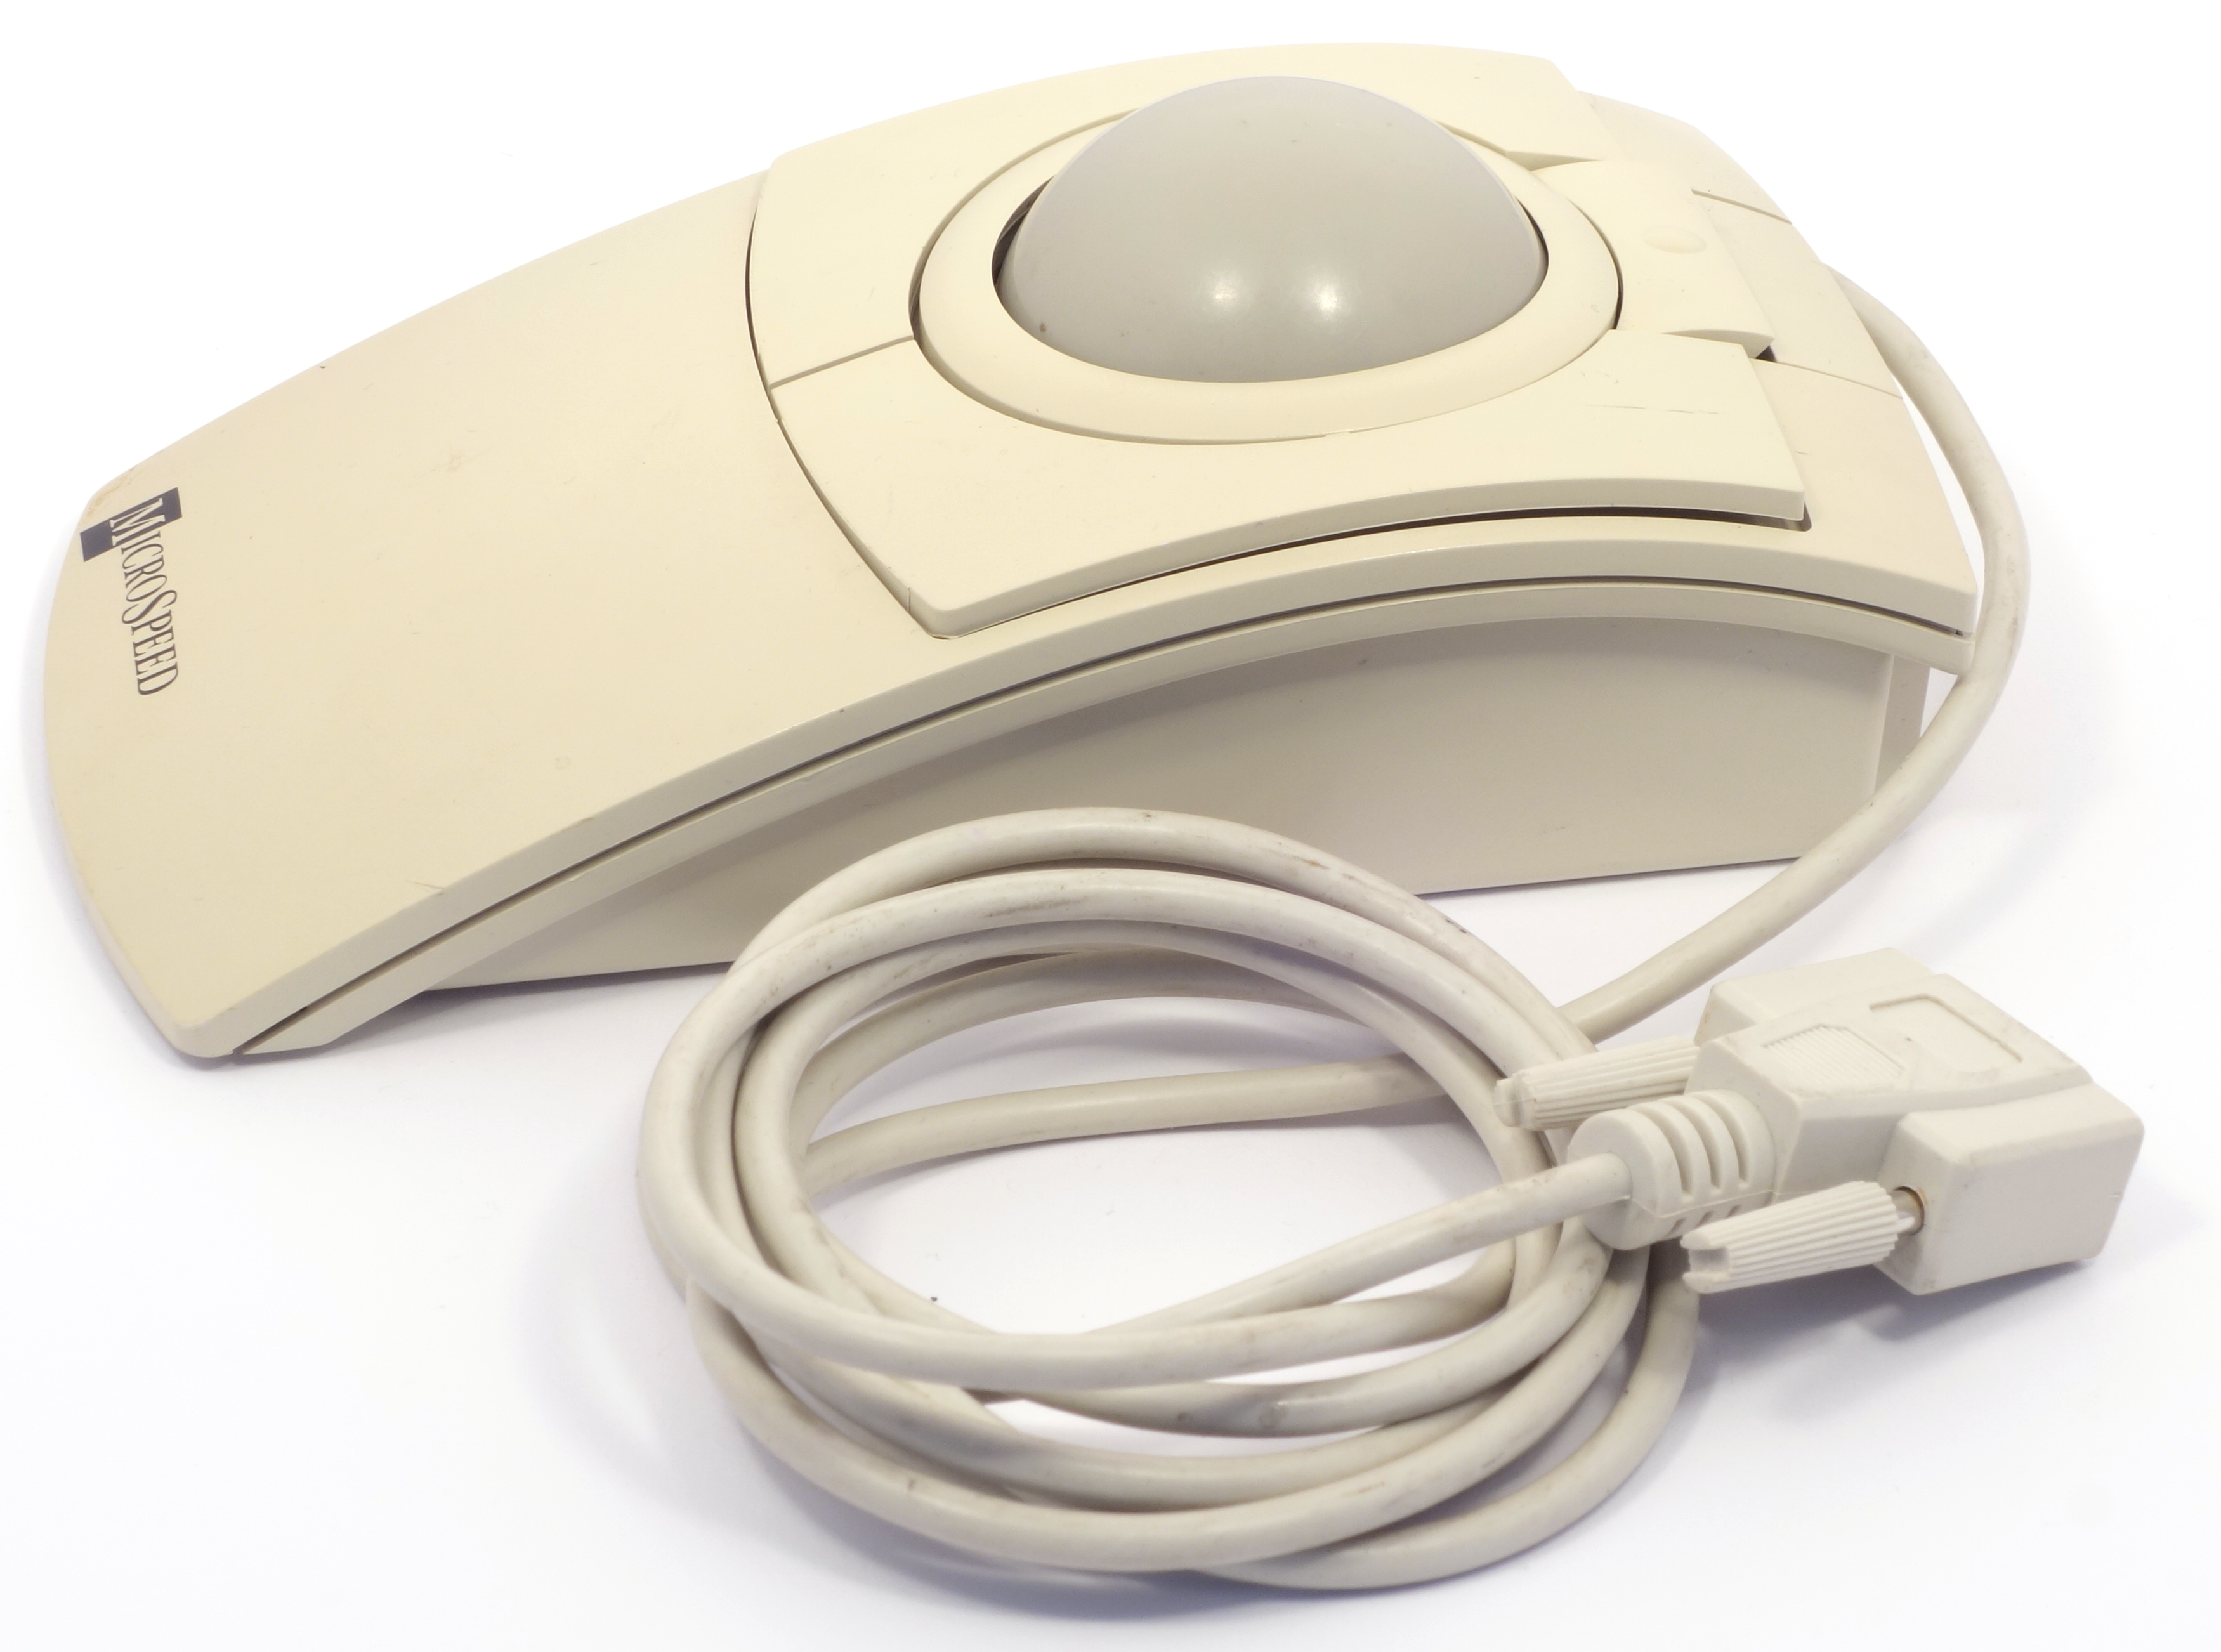
\includegraphics[scale=0.4]{1991_microspeed_pc-track/pic_30.jpg}
    \caption{Изображение трекбола PC-TRACK}
    \label{fig:PCTRACKPic}
\end{figure}

Этот трекбол имеет симметричный дизайн, подходящий как для правшей, так и для левшей (рис. \ref{fig:PCTRACKTopBottom}). 

\begin{figure}[h]
    \centering
    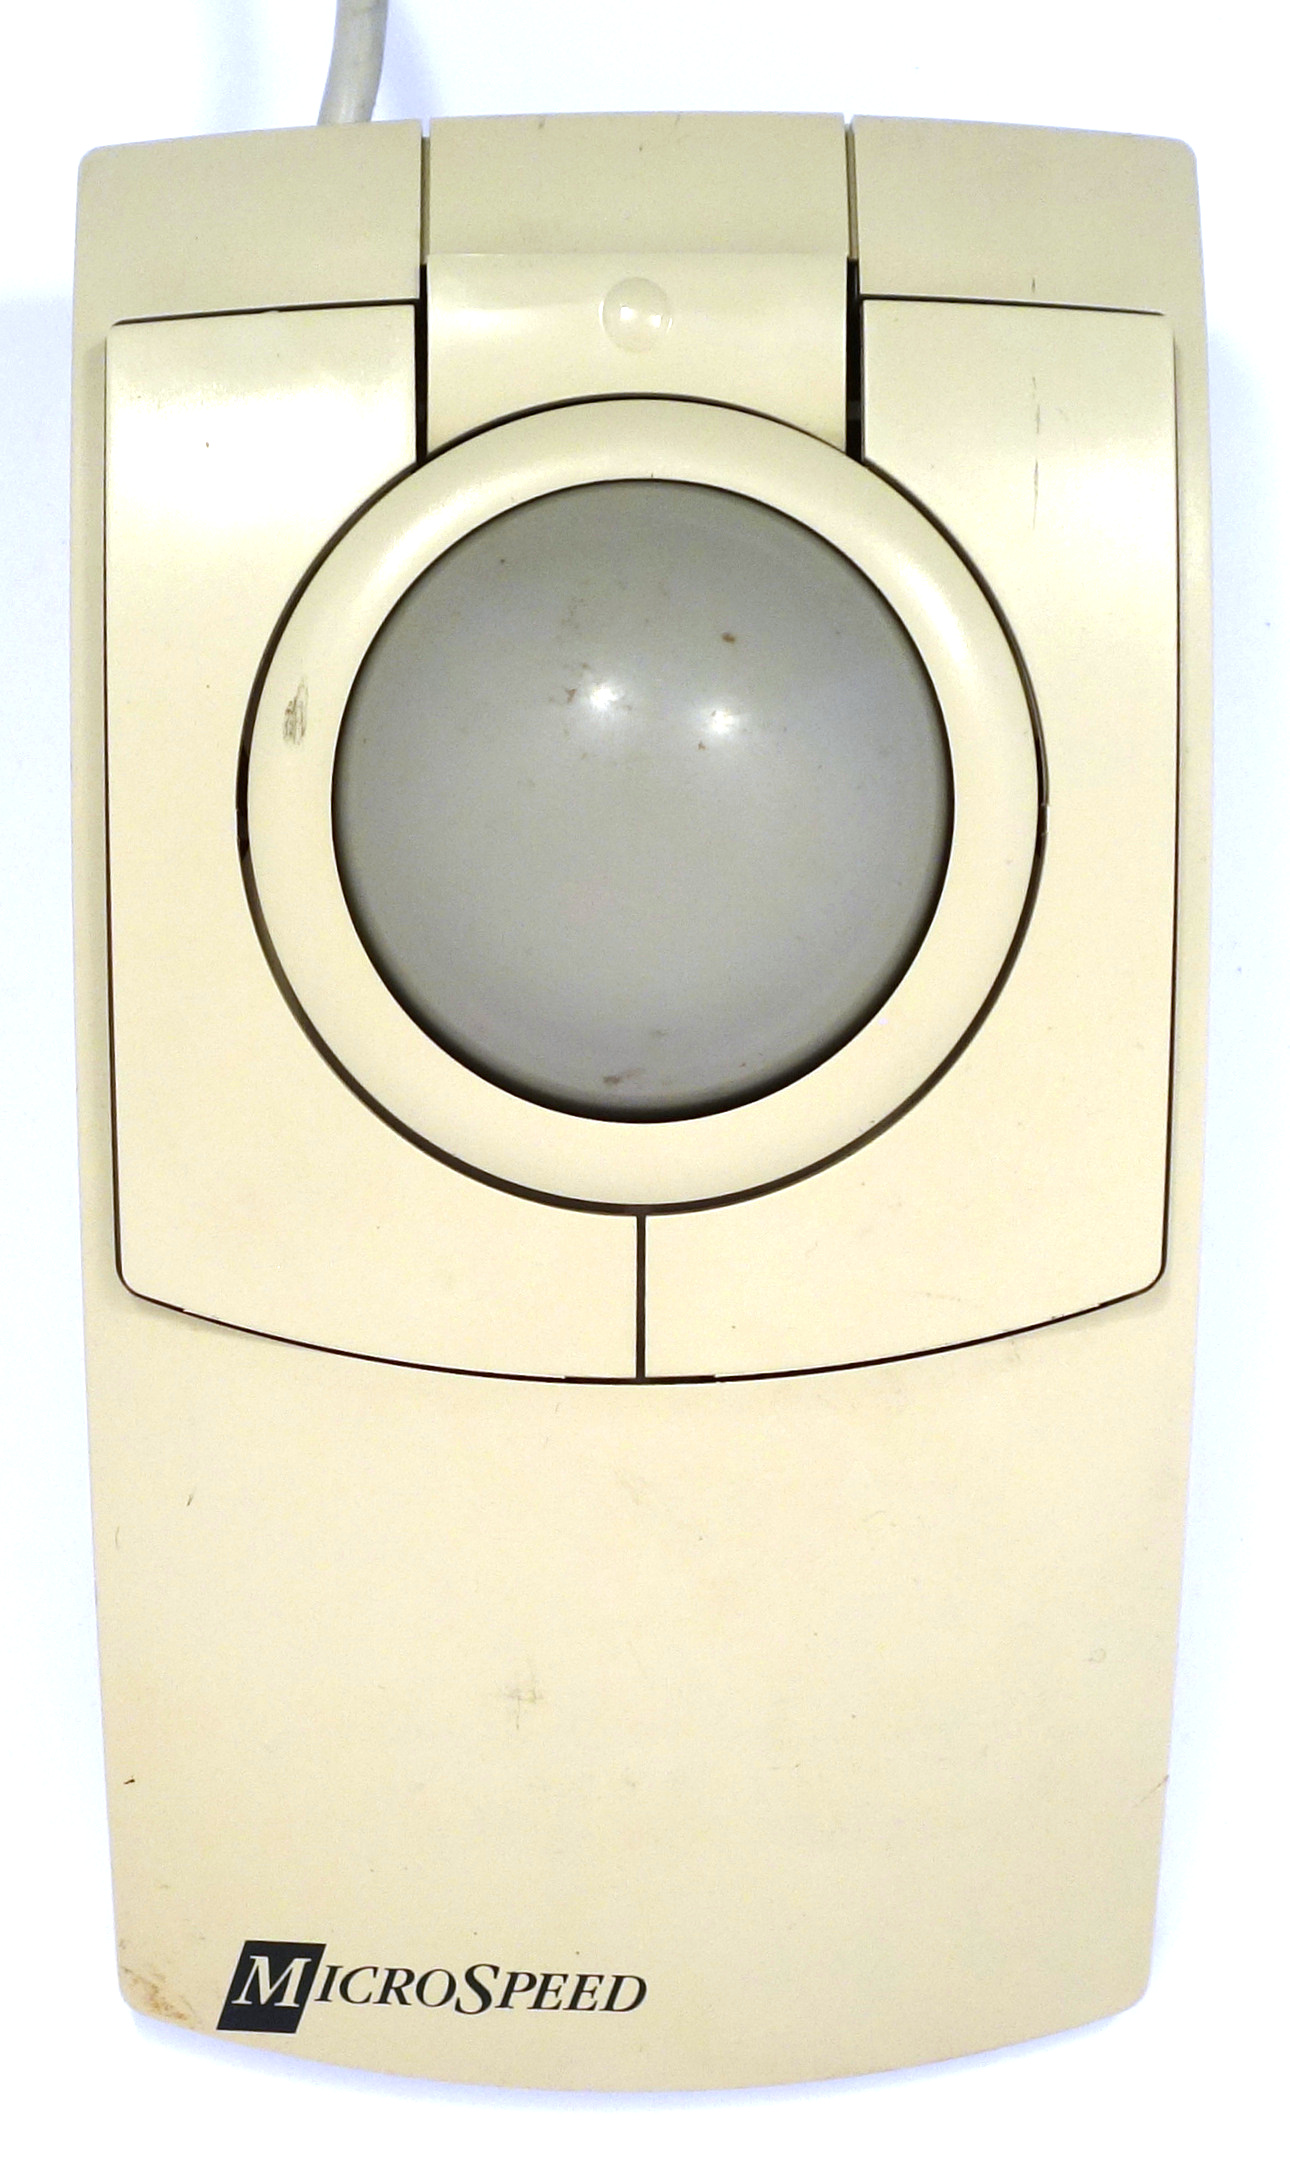
\includegraphics[scale=0.45]{1991_microspeed_pc-track/top_60.jpg}
    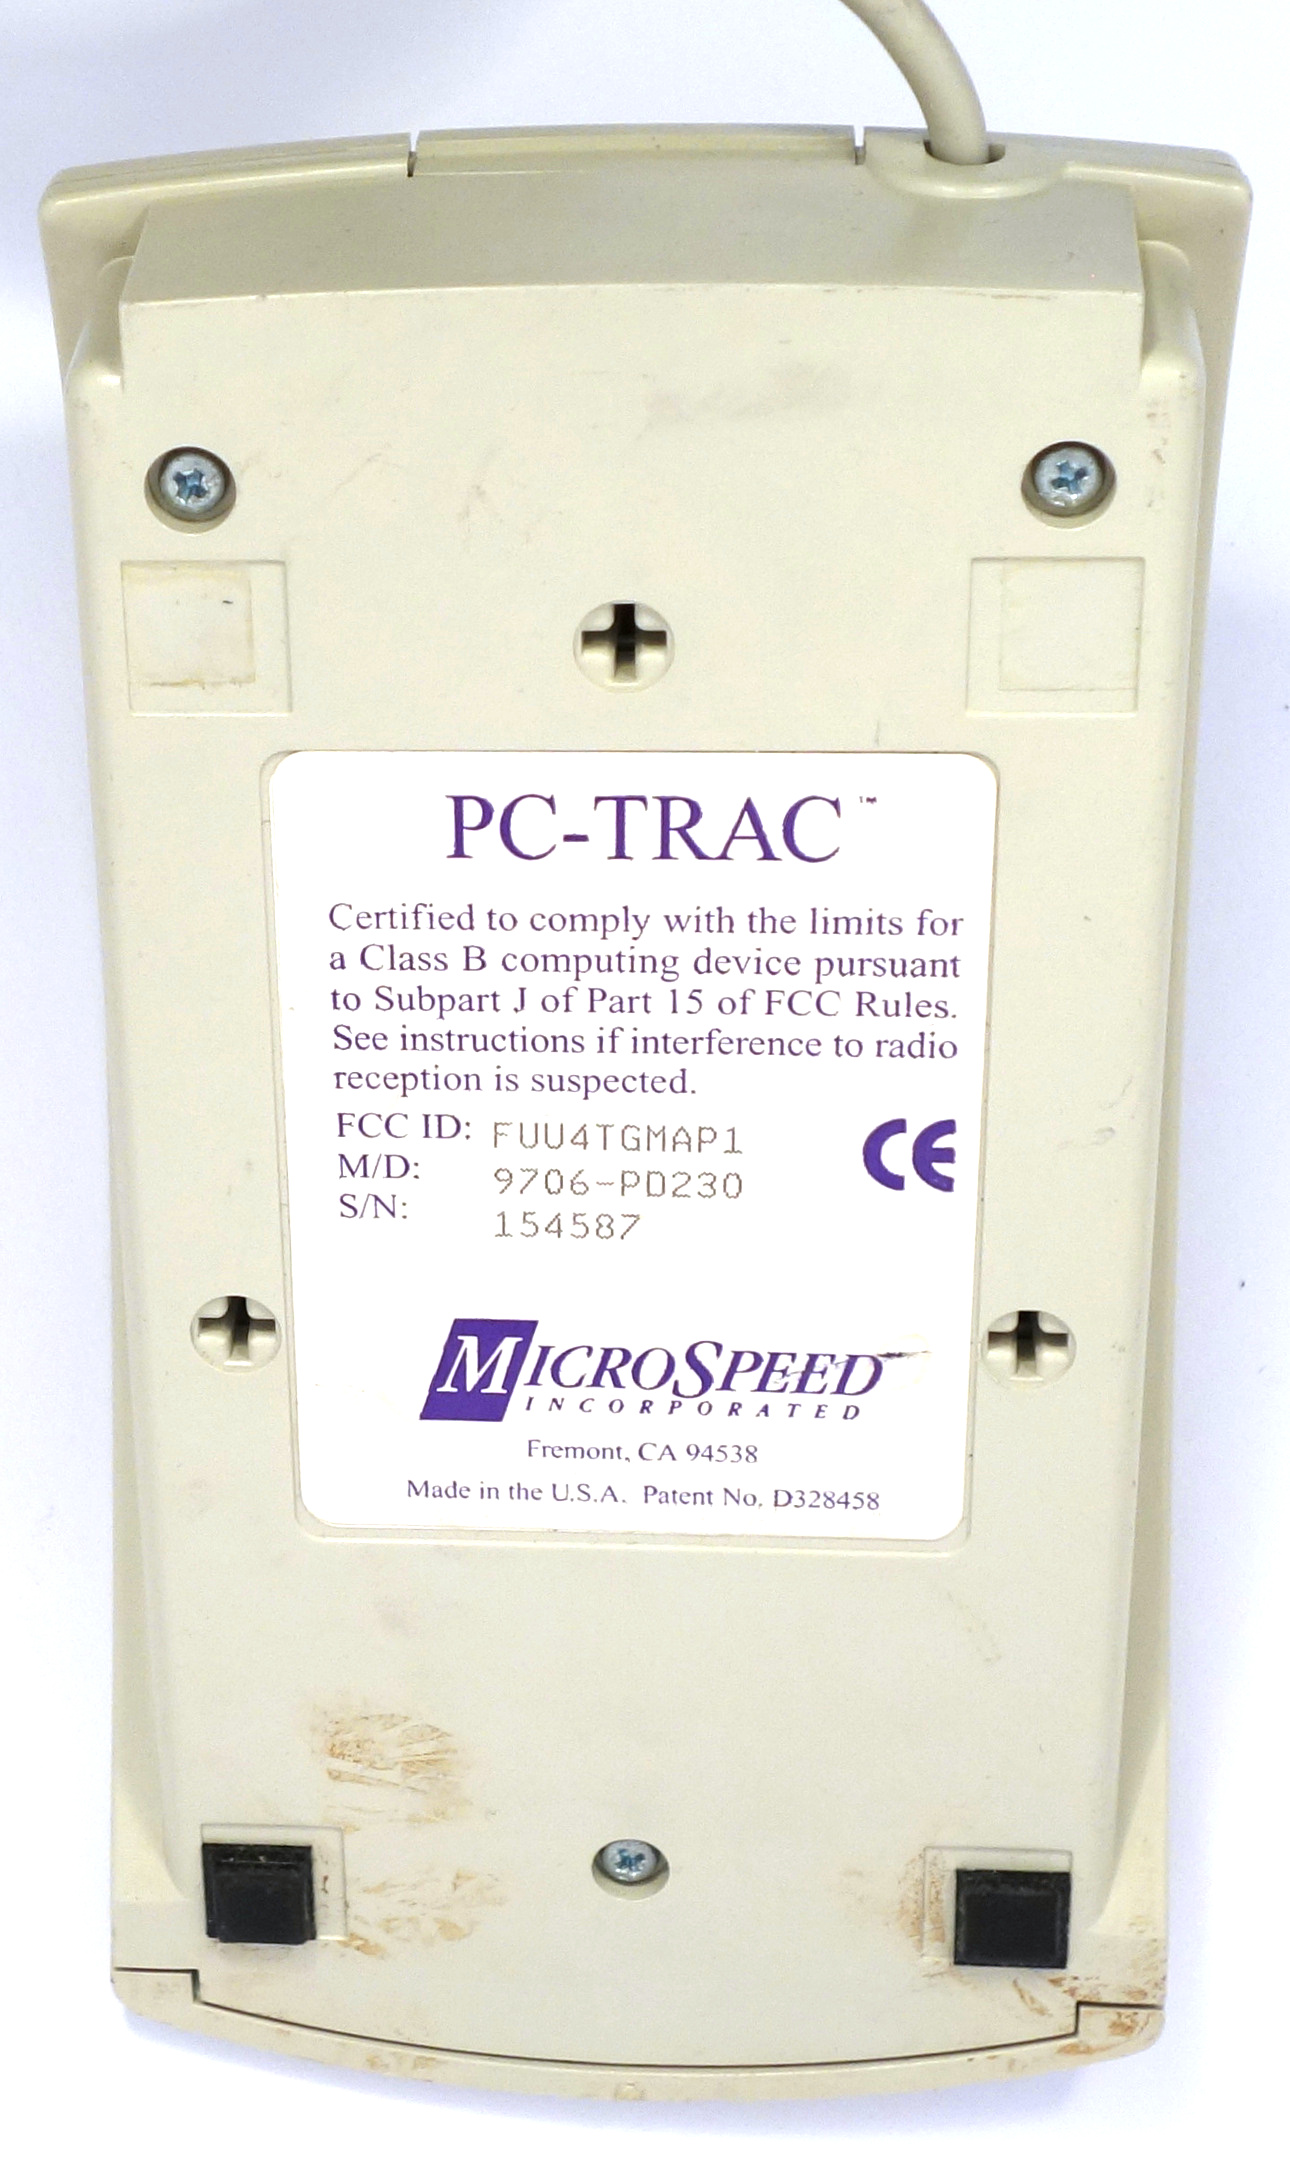
\includegraphics[scale=0.45]{1991_microspeed_pc-track/bottom_60.jpg}
    \caption{Fellowes Trackball, вид сверху и снизу}
    \label{fig:PCTRACKTopBottom}
\end{figure}

Трекбол является крупным (рис. \ref{fig:PCTRACKSize}). MicroSpeed выбрала для данного устройства шар диаметром 2.25 дюйма, потому что их исследования показали значительное увеличение точности позиционирования курсора шаром большего диаметра. Исследования также показали, что лучшей точности способствует и больший вес шара; поэтому примененный 2.25-дюймовый шар обладает на 30 процентов большим весом, чем 2-дюймовый шар, и на 70 процентов большим, чем 1.5-дюймовый шар других моделей.

\begin{figure}[h]
    \centering
    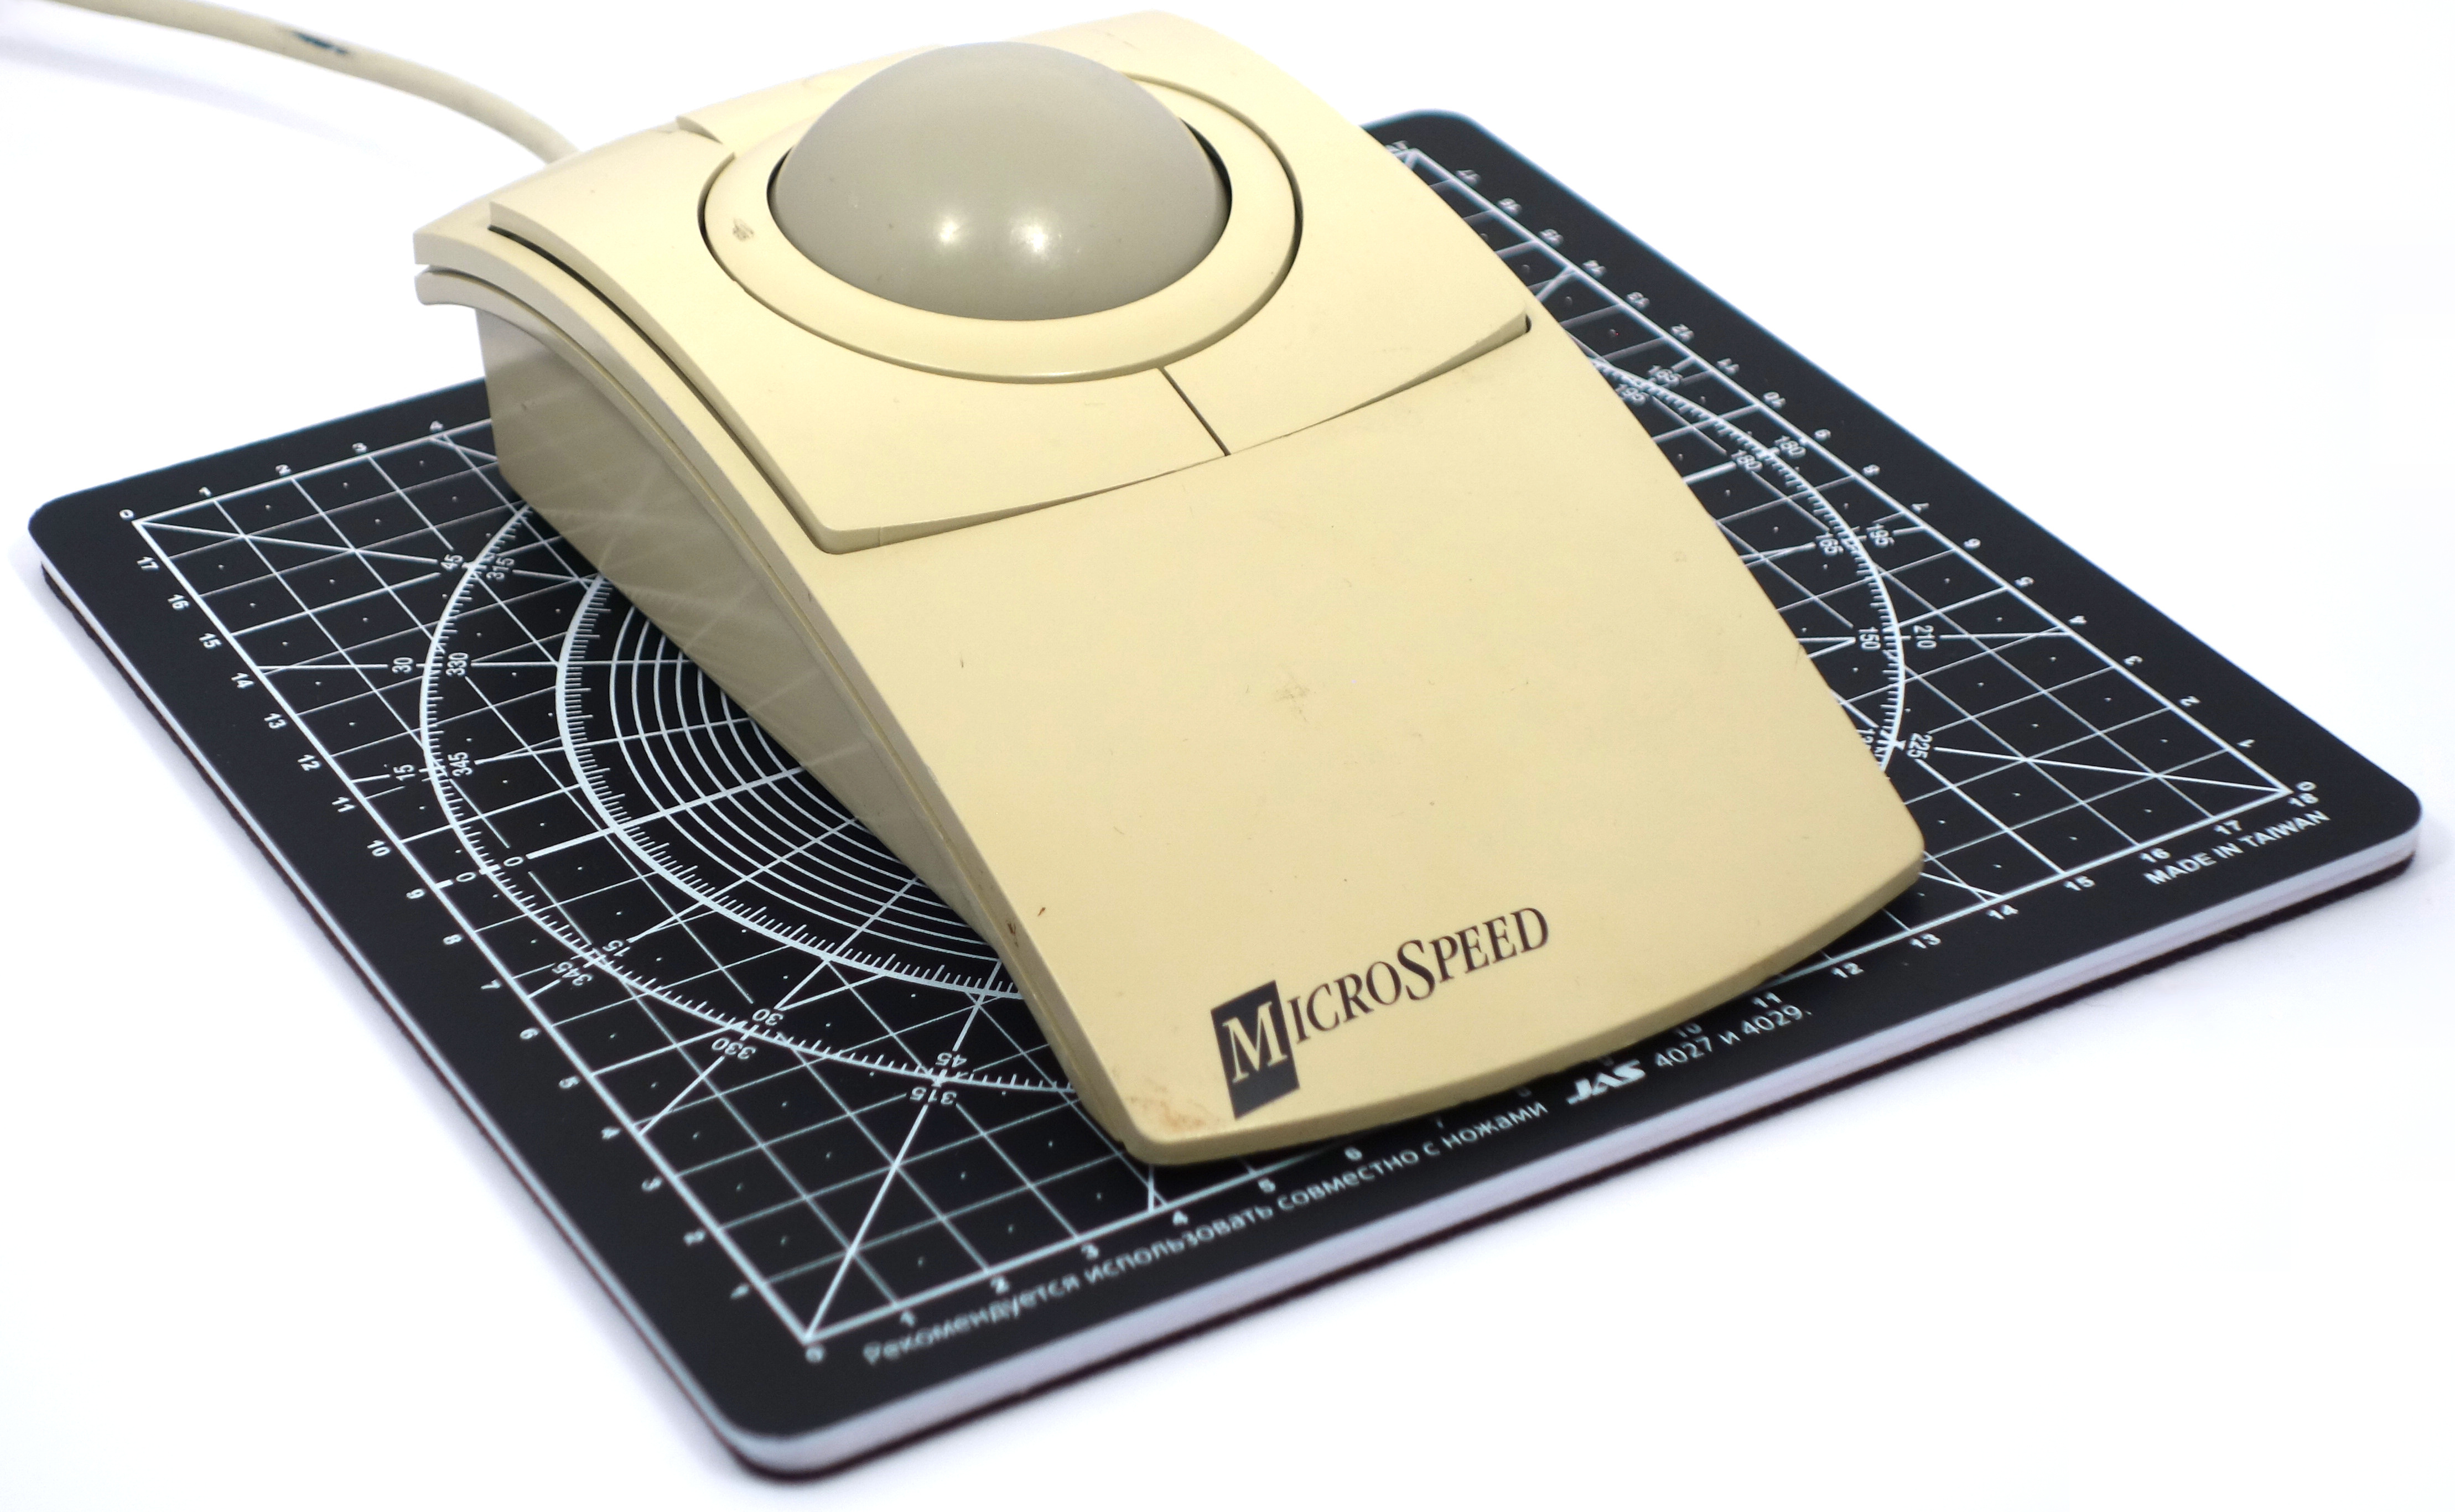
\includegraphics[scale=0.3]{1991_microspeed_pc-track/size_60.jpg}
    \caption{Изображение PC-TRACK на размерном коврике с шагом сетки 1 см}
    \label{fig:PCTRACKSize}
\end{figure}

По бокам шар огибается крупными выпуклыми кнопками, и дополнительно за шаром расположена третья кнопка меньшего размера. Такое расположение основных кнопок является для трекбола более чем удобным; поскольку левая и правая кнопки имеют большую площадь, пользователь может перемещать шар ладонью или подушечками пальцев, а большой палец и мизинец использовать для нажатия на кнопки. Кроме того, этот вариант является симметричным, поэтому одинаково хорошо подходит как для правшей, так и для левшей \ref{fig:PCTRACKHand}. Выпуклая форма PC-TRAC спроектирована таким образом, чтобы соответствовать естественному изгибу руки. Ближняя к пользователю часть корпуса фактически сливается с поверхностью стола, что, согласно заявлению производителя, устраняет присутствовавшую в более ранних конструкциях ступеньку, уменьшая тем самым нагрузку на запястье \cite{PC}.

\begin{figure}[h]
    \centering
    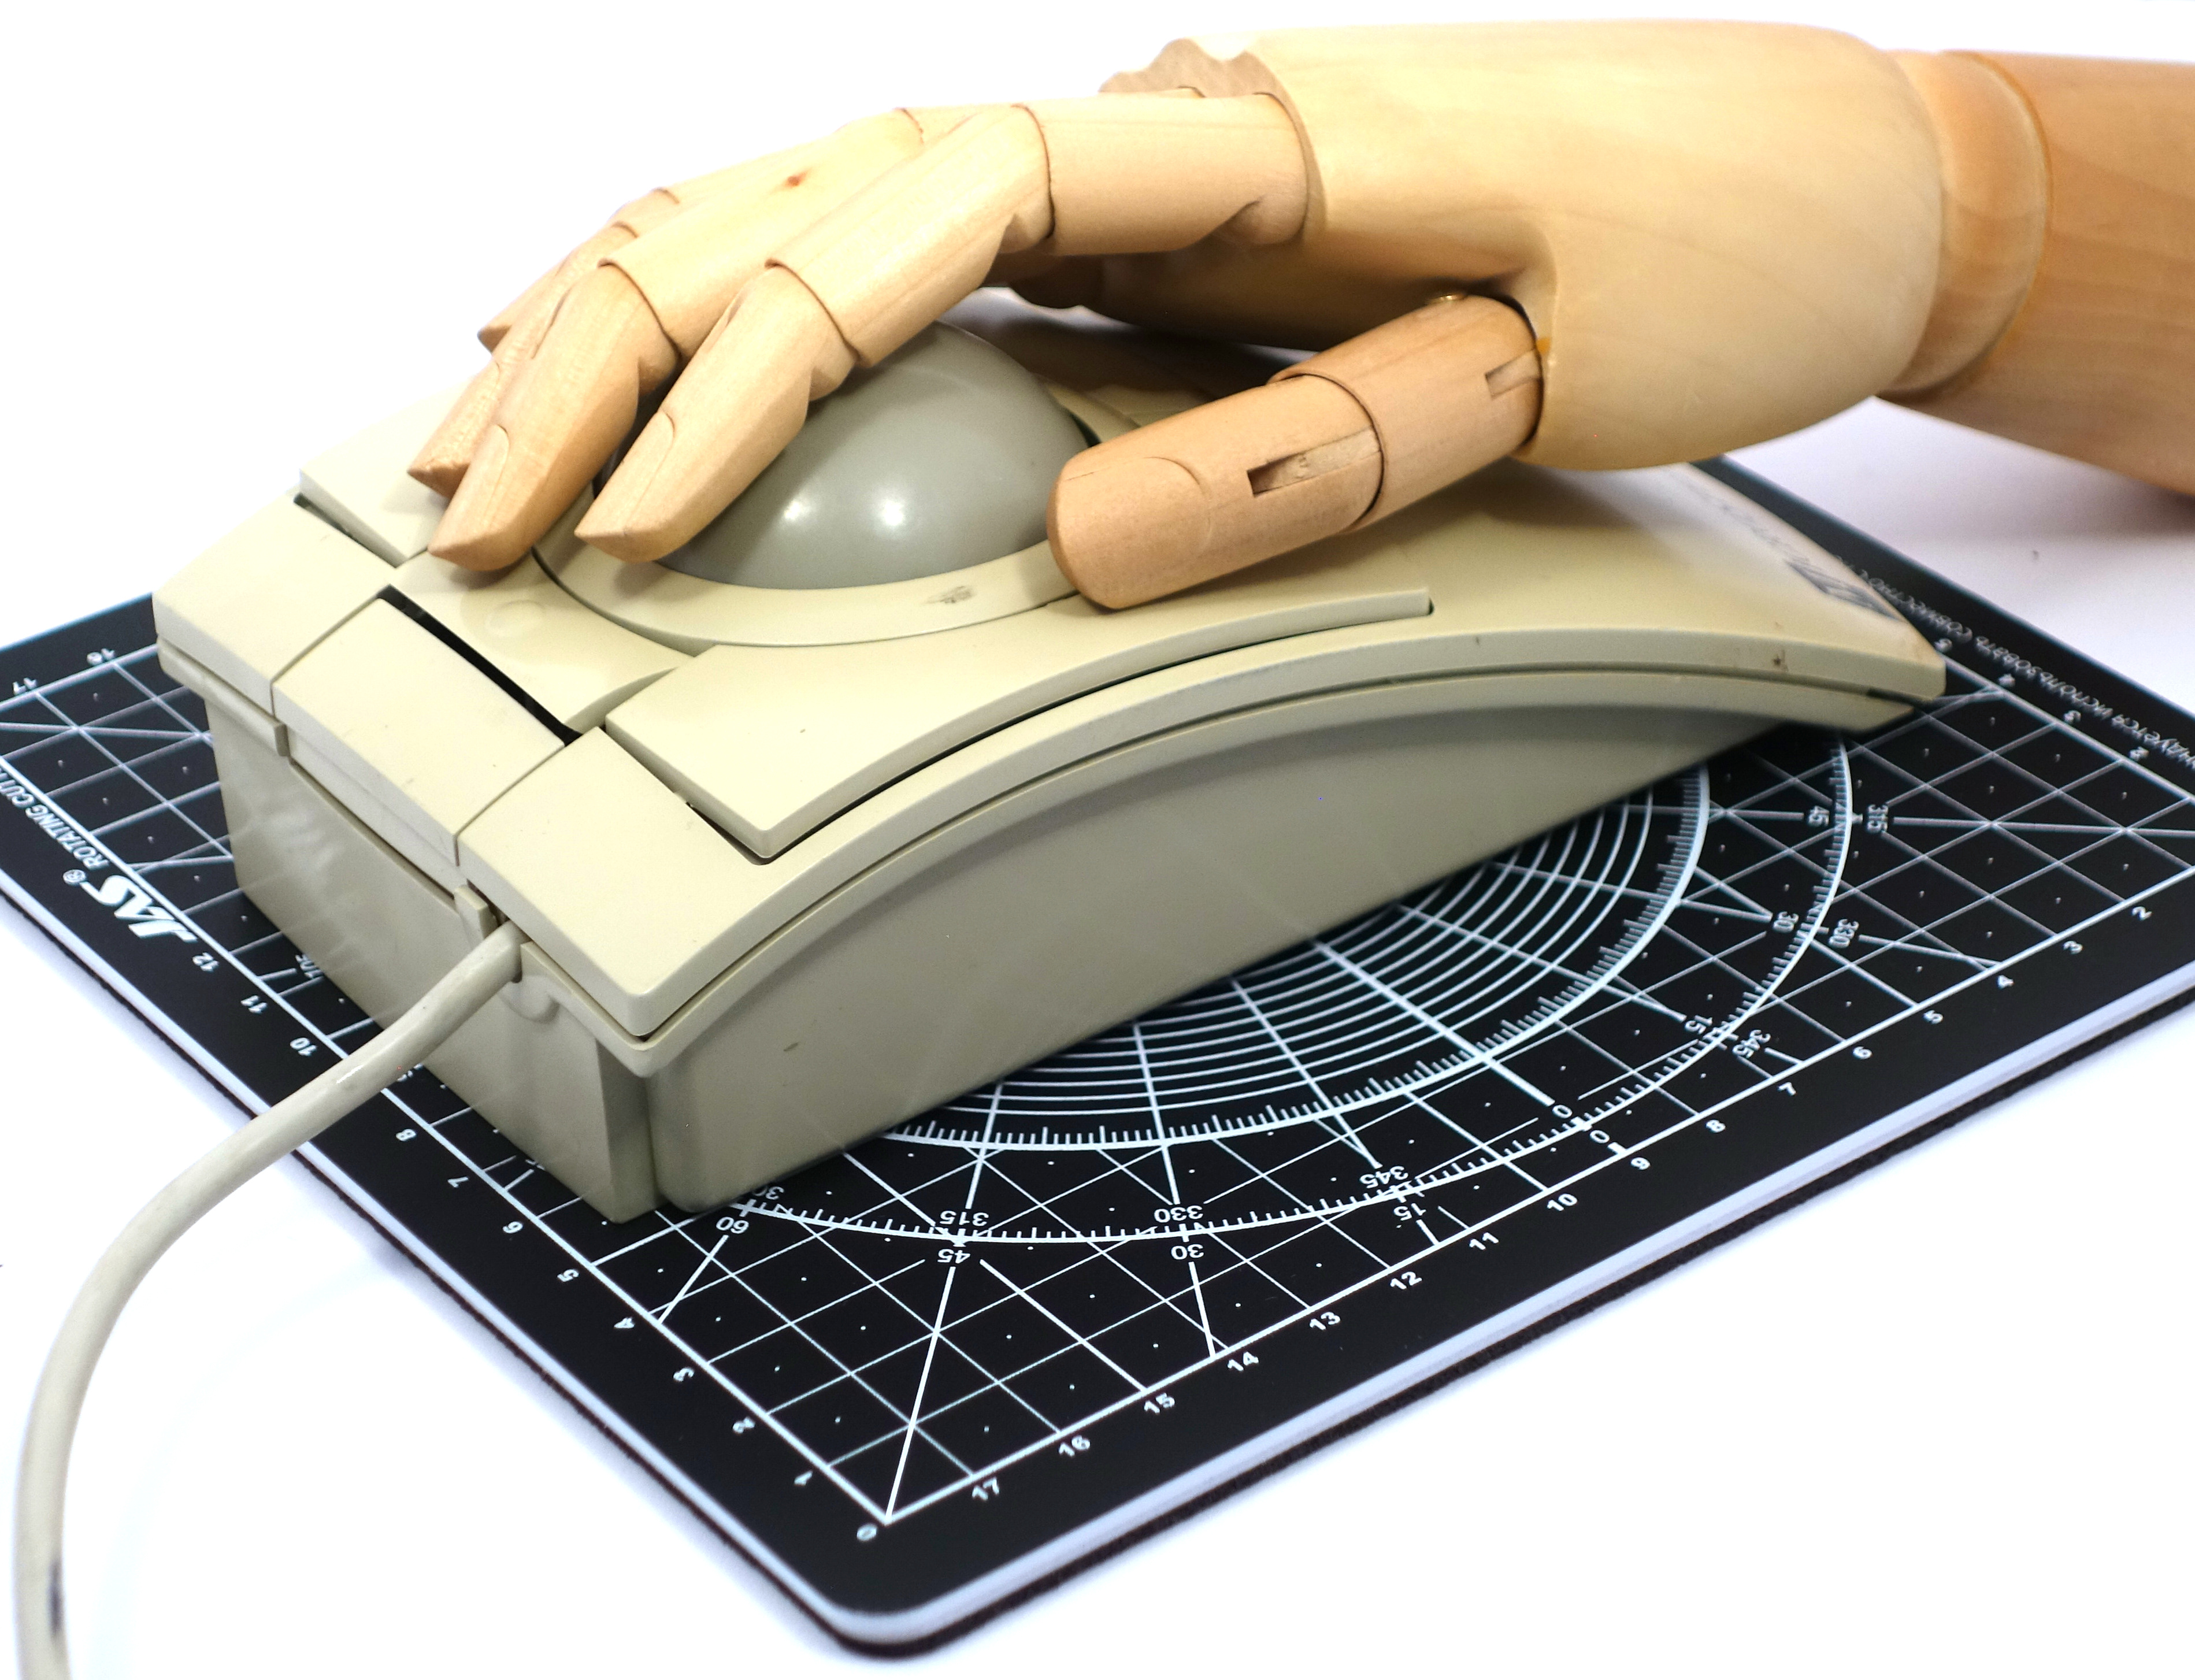
\includegraphics[scale=0.3]{1991_microspeed_pc-track/hand_60.jpg}
    \caption{Изображение PC-TRACK с моделью руки человека}
    \label{fig:PCTRACKHand}
\end{figure}

Меньшая по размеру третья кнопка может использоваться как средняя кнопка мыши или действовать как блокировка перетаскивания. Одна из основных проблем при использовании трекболов с графическими интерфейсами, такими как Windows, на рубеже 80-х и 90-х годов виделась в том, что пользователю сложно перемещать указатель, удерживая нажатой кнопку. Если включена функция блокировки перетаскивания, можно нажать среднюю кнопку после того, как указатель спозиционирован на начальной позиции, переместить указатель к конечной позиции и снова нажать среднюю кнопку, чтобы закончить перетаскивание объекта (с точки зрения компьютера, пользователь все это время удерживал кнопку нажатой). В дополнение к этой функции PC-TRAC также имеет аккордный режим, который позволяет имитировать удерживание обеих кнопок при перемещении мыши.

С точки зрения программного обеспечения трекбол полностью совместим с драйвером мыши Microsoft. Включенные в комплект поставки драйверы PrecisionPointer для DOS и Windows предлагают ряд улучшений, специфичных для трекбола, таких как ускорение при движении курсора (расстояние, на которое перемещается указатель, зависит от того, как быстро вы вращаете шар). Также в комплект входит утилита переназначения клавиш, драйвер для консольных приложений, имитирующий срабатывание курсорных клавиш при вращении шара, а также отдельный драйвер для игры в Тетрис.

\begin{figure}[h]
    \centering
    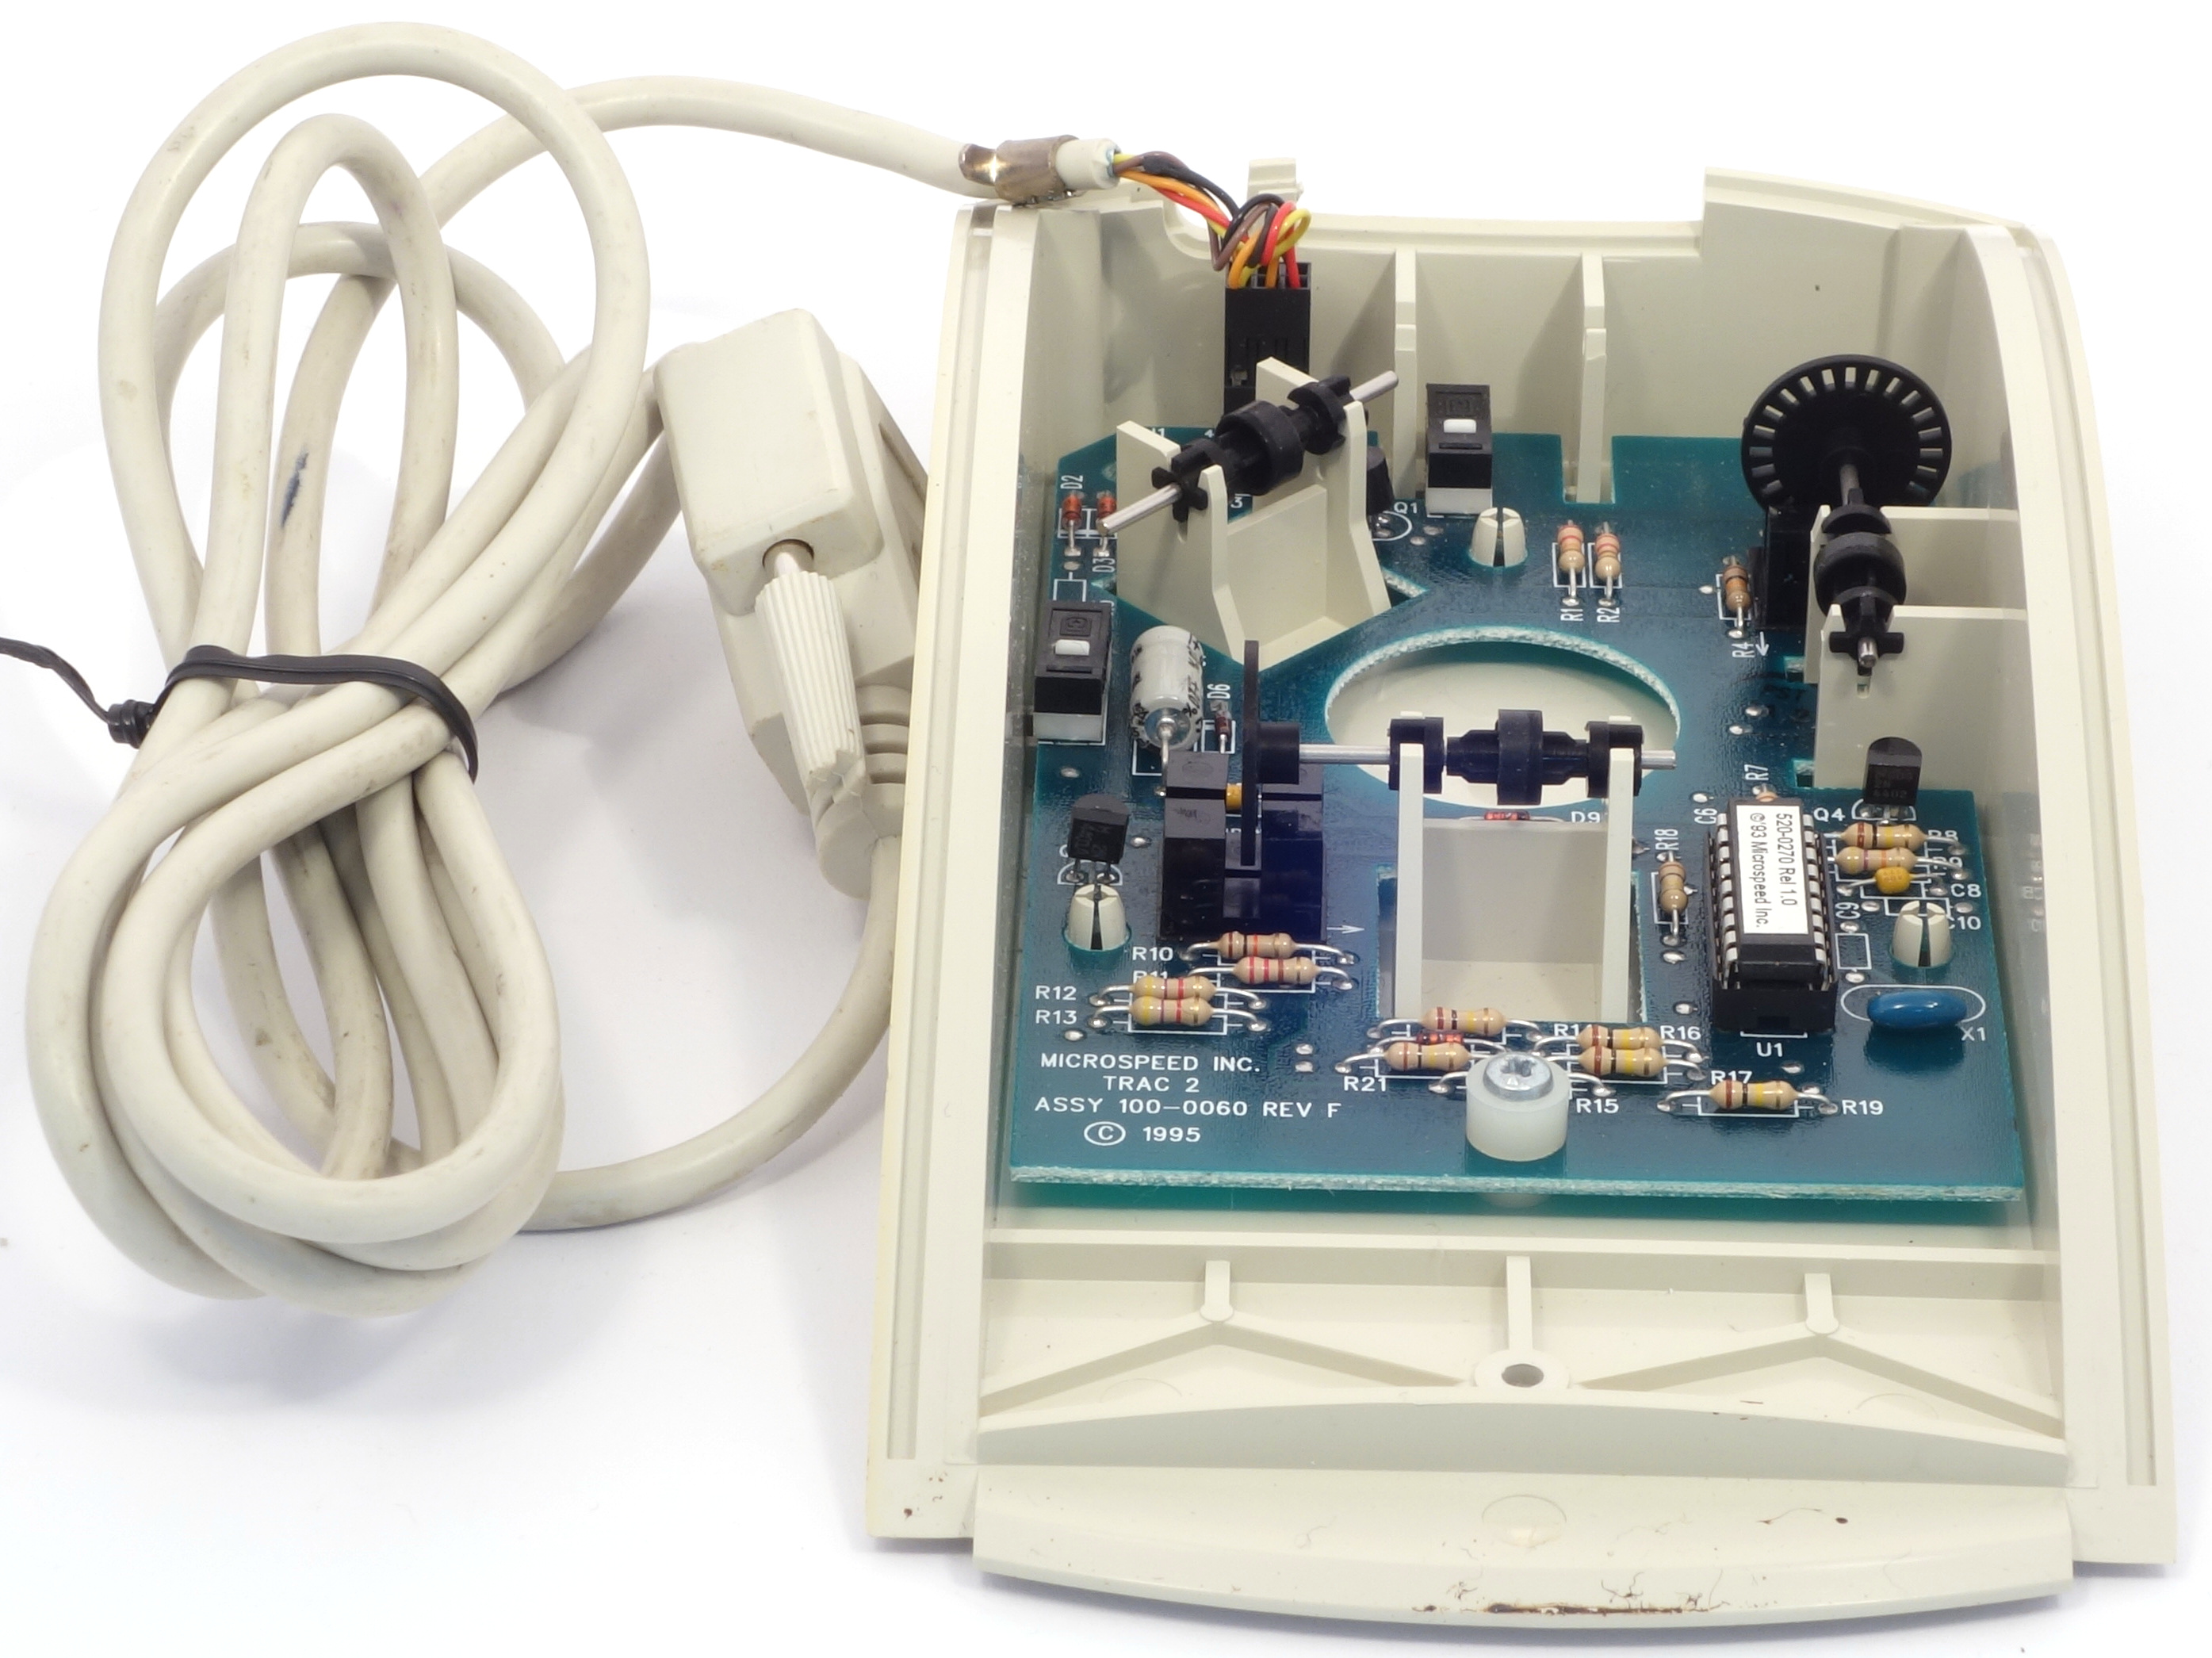
\includegraphics[scale=0.7]{1991_microspeed_pc-track/inside_30.jpg}
    \caption{Изображение PC-TRACK в разобранном виде}
    \label{fig:PCTRACKInside}
    \end{figure}

Рисунок \ref{fig:PCTRACKInside} показывает, что трекбол PC-TRACK выполнен по классической оптомеханической схеме. В конструкции роликов MicroSpeed использовала подшипники качения, изготовленные из пластика Delrin. В рекламных материалах отмечалось, что помимо того, что они являются самосмазывающимися, они более устойчивы, чем металлические подшипники, к образованию каверн, загрязнению и повреждениям в результате механических ударов (например, при падении).

\begin{thebibliography}{9}
\bibitem {PC} MiCROSPEED PC-TRACK // Compute! Magazin,  Iss. 132, August 1991. - p. 50.
\end{thebibliography}
\end{document}
